\documentclass[11pt]{report}
\usepackage{graphicx}
\usepackage{float}
\usepackage{amsmath}
\title{EE312 Diode Transistor Logic}
\date{2018\\ April}
\author{Nail Tosun - 2094563\\ Electric and Electronic Engineering Departmant, METU}
\begin{document}
\maketitle
\section*{Motivation}
To solve the fan-out limitation of RTL when output HIGH case.
\begin{figure}[H]
  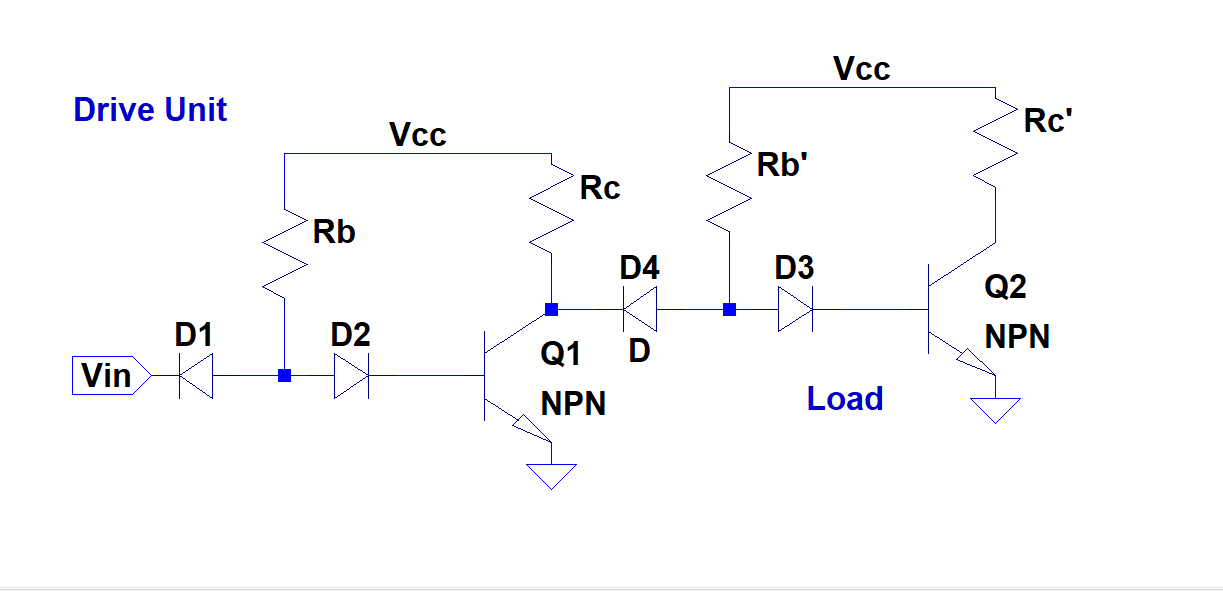
\includegraphics[width=\linewidth]{dtl}
  \caption{Diode Transistor Logic Inverter Circuit}
  \label{fig:zero}
\end{figure}
Due to the fact that existence of D1 and D4 diodes, when $V_{Q1_c}$ is high (meaning that output high) there is no sinking current to the driver unit therefore output high fan-out is significantly improved. 
\section*{Voltage Transfer Characteristic}
\[ \begin{cases} 
      5 & 0 \leq V_{in}\leq 0.7 \\
      -\frac{4.8V_{in}}{0.1} & 0.7 \leq x\leq 0.8 \\
      0.2 & 0.8 \leq x \leq 5 
   \end{cases}
\]
\end{document}